
\section{Recap}


\begin{frame}{Variational auto-encoder}

Generative model with NN likelihood

~

\begin{columns}
	\begin{column}{0.2\textwidth}
	\begin{tikzpicture}
    % Define nodes
    \node[latent]		(z)		{$ z $};
    \node[obs, below = of z]		(x)		{$ x $};
    \node[right = of x]		(theta)		{$ \theta $};
    
    % Connect nodes
    \edge{z,theta}{x};
    
    % add plates
    \plate {x-sentence} {(x)(z)} {$ N $};
   
    \node[right = of z]		(lambda)		{$ \lambda $};   
    \edge[dashed, bend right]{x}{z};
    \edge[dashed]{lambda}{z};
    \end{tikzpicture}
    \end{column}
    \begin{column}{0.7\textwidth}
    	\begin{itemize}
			\item complex (non-linear) observation model $p_\theta(x|z)$
			\item complex (non-linear) mapping from data to latent variables $q_\lambda(z|x)$
    	\end{itemize}
    \end{column}
    \end{columns}
    ~
    
    Jointly optimise generative model $p_\theta(x|z)$ and inference model $q_\lambda(z|x)$ under the same objective (ELBO)
    
    \ack{\citet{KingmaWelling:2013}}
\end{frame}


\begin{frame}[plain]{Objective}

\begin{equation*}
\begin{aligned}
\log p_\theta(x) &\geq \overbrace{\E[q_\lambda(z|x)]{\log p_\theta(x|Z)} - \KL{q_\lambda(z|x)}{p(z)}}^{\ELBO} 
\end{aligned}
\end{equation*}

\pause

Parameter estimation
\begin{equation*}
\argmax_{\theta,\lambda} ~ \E[q(\epsilon)]{\log p_\theta(x|\underbrace{h^{-1}(\epsilon, \lambda)}_{=z})} - \KL{q_\lambda(z|x)}{p(z)}
\end{equation*}

\pause

\begin{itemize}
	\item assume $\KL{q_\lambda(z|x)}{p(z)}$  analytical\\
	true for exponential families \pause
	\item approximate $\E[q(\epsilon)]{\log p_\theta(x|h^{-1}(\epsilon, \lambda))}$ by sampling\\
	requires a reparameterisation $h^{-1}(\epsilon, \lambda) \sim q_\lambda(z|x)  \Leftrightarrow  h(z, \lambda) \sim q(\epsilon)$
\end{itemize}


\end{frame}

\section{Discrete variables}

\begin{frame}{Discrete variables}

Suppose $z$ is a $d$-dimensional binary vector \\
\quad i.e. $z_i \in \{0, 1\}$ \\

~ \pause

Then let's define an inference model
\begin{equation}
q_\lambda(z|x) = \underbrace{\prod_{i=1}^d q_\lambda(z_i|x)}_{\text{mean field}} \pause =  \prod_{i=1}^d \Bern(z_i|\underbrace{\sigmoid(f_\lambda(x))}_{\text{NN}})
\end{equation}


\pause

\textcolor{blue}{Can we reparameterise $q_\lambda(z_i|x)$? }


\end{frame}

\begin{frame}{Bernoulli pmf}

\begin{equation}
\begin{aligned}
\Bern(z_i|b_i) &= b_i^{z_i} (1 - b_i)^{1 - z_i} \pause \\
&= 
\begin{cases}
b_i & \text{if } z_i = 1 \\
1-b_i & \text{if } z_i = 0
\end{cases}
\end{aligned}
\end{equation}

\pause

\textcolor{blue}{Can we reparameterise a Bernoulli variable?}



\end{frame}

\begin{frame}{Reparameterisation requires a Jacobian matrix}


\alert{Not really :(} 

\begin{equation}
\begin{aligned}
q(z; \lambda) = \underbrace{\phi(\epsilon = h(z, \lambda)) \abs{\det \alert{J_{h(z, \lambda)}}}}_{\text{change of density}}
\end{aligned}
\end{equation}


Elements in the Jacobian matrix 
$$J_{h(z, \lambda)}[i,j] = \pdv{h_i(z, \lambda)}{z_j}$$
are not defined for non-differentiable functions


\end{frame}

\section{Continuous relaxation}

\begin{frame}{Relaxation}

Let's redefine $z_i$ to live in the interval $(0,1)$
\begin{itemize}
	\item and find an alternative reparameterisable {\bf density}\\
\end{itemize}

\pause

Examples
\begin{itemize}
	\item $Z \sim \mathcal {LN}(u, s^2)$\\
	$z = \sigmoid(u +  s\epsilon)$ with $\epsilon \sim \mathcal N(0, 1)$ \pause	
	\item $Z \sim \Kuma(a, b)$\\
	$z = \left(1 - (1 - \epsilon)^{\frac{1}{b}}\right)^{\frac{1}{a}}$ with $\epsilon \sim \mathcal U(0,1)$ \pause
	\item $Z \sim \Concrete(u, \tau)$\\
	$z= \sigmoid(\frac{u + \epsilon}{\tau})$ with $\epsilon \sim \Gumbel(0, 1)$ 
\end{itemize}

~ \pause

But note that we {\bf no longer} have a discrete variable

\ack{\beamerbutton{\href{https://en.wikipedia.org/wiki/Kumaraswamy_distribution}{Kumaraswamy}} ~ \beamerbutton{\href{https://en.wikipedia.org/wiki/Gumbel_distribution}{Gumbel}}}
	
\end{frame}

\begin{frame}{Straight-through estimator}

Let $\sigma: (0,1) \rightarrow \{0,1\}$ map from a continuous relaxation $z$ to a discrete sample, e.g.
\begin{equation}
\sigma(z) = 
\begin{cases}
1 & \text{if }z > 0.5 \\
0 & \text{otherwise}
\end{cases}
\end{equation}

\pause

Then we compute a forward pass with the discrete variable
\begin{equation}
 \E[q(\epsilon)]{\log p_\theta(x|\sigma(\underbrace{h^{-1}(\epsilon, \lambda)}_{=z}))}
 \end{equation} \pause
but back-propagate through the continuous relaxation
\begin{equation}
\pdv{\sigma(h^{-1}(\epsilon, \lambda))}{\lambda} \overset{\text{def}}{=} \pdv{h^{-1}(\epsilon, \lambda)}{\lambda}
\end{equation}

\ack{\citet{bengio2013estimating}}

\end{frame}


\begin{frame}{Stochastic optimisation with ST estimator}

The straight-through estimator is {\bf biased}
\begin{itemize}
	\item and it's bias cannot be quantified analytically 
\end{itemize}

~

Stochastic optimisation with biased gradients is a heuristic
\begin{itemize}
	\item its success will vary from case to case and there are no general lessons
	\item it has been shown to work for 
	\begin{itemize}
		\item simple discrete (binary or 1-of-K) variables \citep{jang2016categorical}
		\item for sequences \citep{havrylov2017emergence}
	\end{itemize}
	\item but for trees the story is not as clear \citep{choi2017learning}
\end{itemize}

\end{frame}

\begin{frame}{Concrete or Gumbel-Softmax}

An alternative parameterisation of a Categorical variable
\begin{equation}
\begin{aligned}
A &\sim \Cat(\softmax(\phi)) \\
A &= \argmax_i ~ \left[\phi_i + \epsilon_i\right]_{i=1}^{K} \quad \text{where } \epsilon \sim \Gumbel(0, I)
\end{aligned}
\end{equation}

\pause

We can sample a one-hot encoding of the categorical variable
\begin{equation}
\begin{aligned}
B &= \onehot\left( \argmax_i ~ \left[\phi_i + \epsilon_i\right]_{i=1}^{K} \right) %\quad \text{where } \epsilon \sim \Gumbel(0, 1)
\end{aligned}
\end{equation}

\pause

And we get a continuous relaxation with $\softmax$
\begin{equation}
\begin{aligned}
B &= \softmax (\phi + \epsilon) 
\end{aligned}
\end{equation}

\pause

Finally, with a temperature $\tau$ we can approach a one-hot encoding of the most likely category as $\tau \to 0$
\begin{equation}
\begin{aligned}
B &= \softmax \left(\frac{\phi + \epsilon}{\tau} \right) 
\end{aligned}
\end{equation}

\end{frame}

\begin{frame}{Simplex}

The tips of the simplex represent a one-hot encoding of a 3-way Categorical variable

\begin{center}
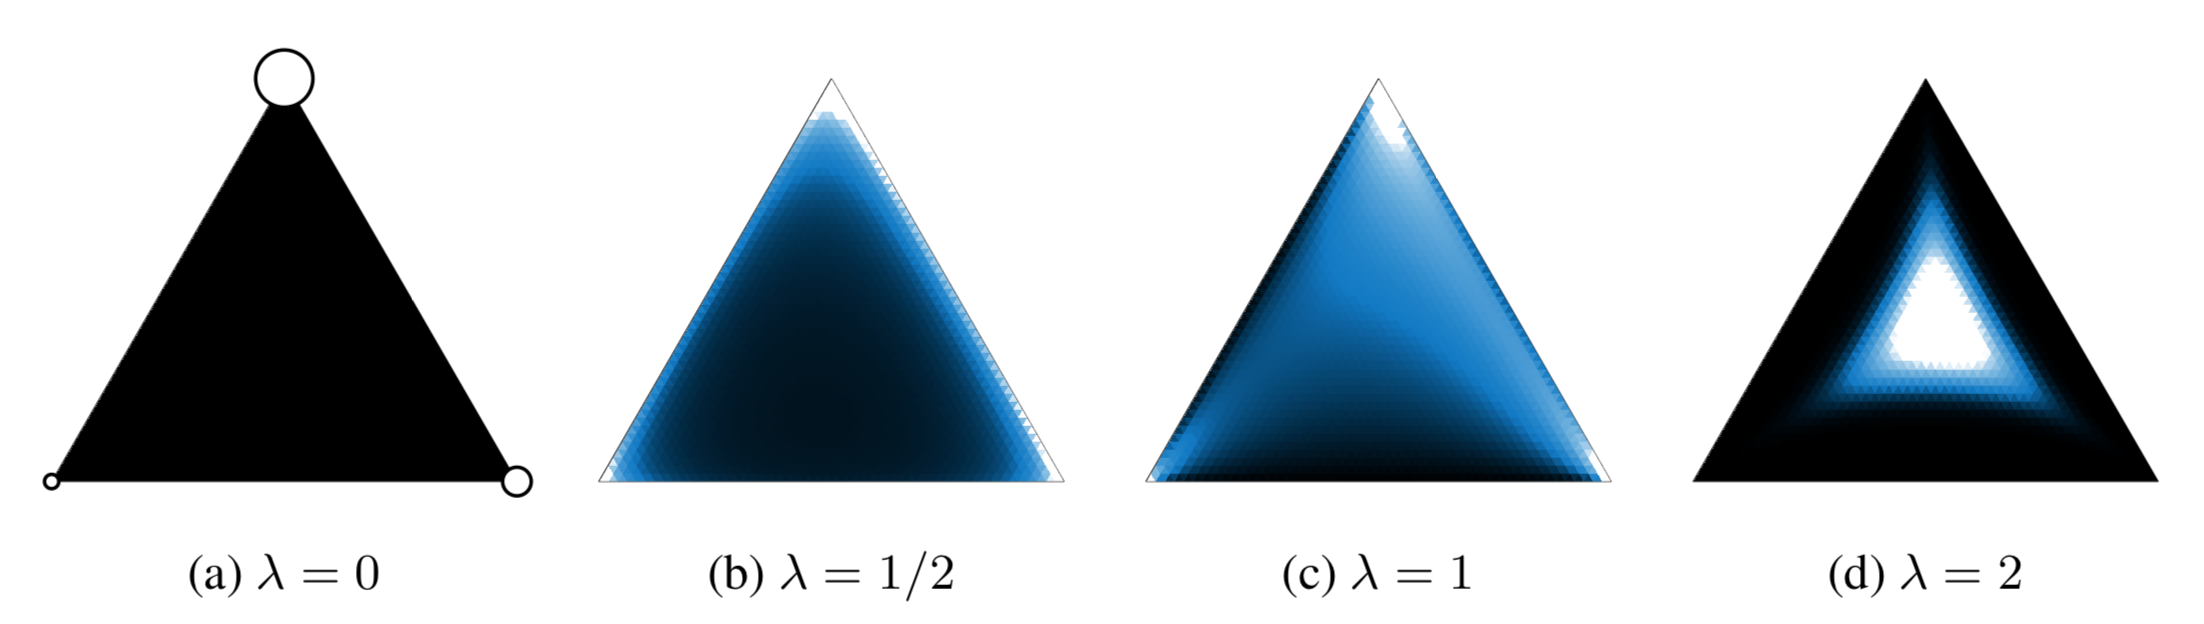
\includegraphics[scale=0.25]{img/simplex}
\end{center}

\begin{itemize}
	\item the $\softmax$ relaxes the variable to take on values in the interior of the simplex
	\item as we cool down the system we push most of the mass towards the tips
\end{itemize}

\ack{Illustrations from  \citep{maddison2016concrete}.}

\end{frame}


\begin{frame}{Concrete samples}

\begin{center}
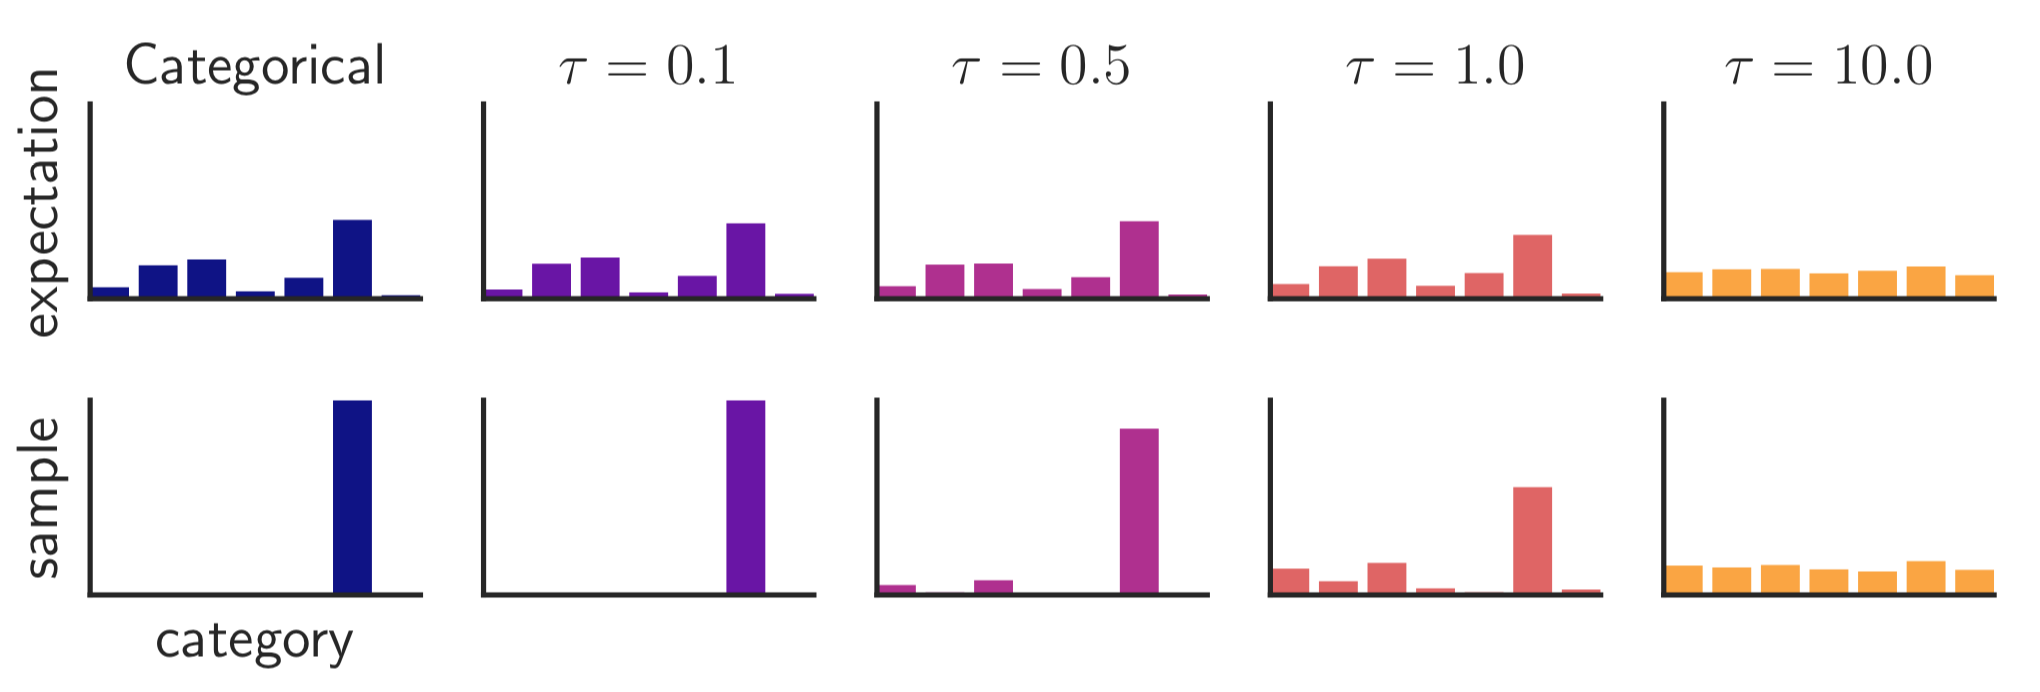
\includegraphics[scale=0.25]{img/bars}
\end{center}


\ack{Illustrations from \citep{jang2016categorical}.}

\end{frame}



